\documentclass[a4paper,man,floatsintext,longtable,noextraspace,12pt]{apa6}

\usepackage[english]{babel}
\usepackage[utf8x]{inputenc}
\usepackage{amsmath}
\usepackage{graphicx}
\usepackage[colorinlistoftodos]{todonotes}
\usepackage{hyperref}

\usepackage{booktabs}
\usepackage{longtable}
\usepackage{array}
\usepackage{multirow}
\usepackage{wrapfig}
\usepackage{float}
\usepackage{colortbl}
\usepackage{pdflscape}
\usepackage{tabu}
\usepackage{threeparttable}
\usepackage{threeparttablex}
\usepackage[normalem]{ulem}
\usepackage{makecell}
\usepackage{xcolor}
% make captions italic

% number lines
% \usepackage{lineno}
% \linenumbers
            
% bibliography
\newlength{\cslhangindent}
\setlength{\cslhangindent}{1.5em}
\newenvironment{CSLReferences}%
  {}%
  {\par}

% tightlist
\providecommand{\tightlist}{%
  \setlength{\itemsep}{0pt}\setlength{\parskip}{0pt}}

\title{\textbf{How open are hybrid journals included in transformative agreements?}}
\shorttitle{Hybrid OA}
\author{Najko Jahn}
\affiliation{Göttingen State and University Library, University of Göttingen\\
Platz der Göttinger Sieben 1, 37073 Göttingen, Germany\\
najko.jahn@sub.uni-goettingen.de
}

\authornote{ORCID: https://orcid.org/0000-0001-5105-1463}

\abstract{The ongoing controversy surrounding transformative agreements, which aim to transition journal publishing to full open access, highlight the need for large-scale studies assessing the uptake of open access in hybrid journals. This includes evaluating the extent to which transformative agreements enabled open access. By combining publicly available data from various sources, including cOAlition S Journal Checker, Crossref, and OpenAlex, this study presents a novel approach that analyses over 700 agreements and nine million journal articles published in more than 11.000 hybrid journals. Estimates suggest a strong growth in open access between 2018 and 2022 from 4.3\% to 15\%. In 2022, 58\% of hybrid open access was enabled by transformative agreements. This trend was largely driven by the three commercial publishers Elsevier, Springer Nature, and Wiley, but the open access uptake varied substantially across journals, publishers, disciplines, and country affiliations. In particular, comparing the developments in the OECD and BRICS areas revealed different publication trends relative to hybrid open access. In conclusion, estimates suggest that current levels of implementation of transformative agreements is insufficient to bring about a large-scale transition to full open access.}

\keywords{hybrid open access, transformative agreements, scholarly publishing, big deals, bibliometrics}

\begin{document}
\maketitle

% QSS wants numbered sections
%\setcounter{secnumdepth}{2}

\hypertarget{introduction}{%
\section{Introduction}\label{introduction}}

For over two decades, hybrid open access journal publishing, which makes
some articles openly available while others remain behind a paywall, has
been discussed as a means for transitioning the subscription system to
full open access (Prosser, 2003). The idea was that when journals
increasingly publish open access articles, they could reduce revenues
from subscriptions, while libraries and funders could change their
funding models and shift expenditures from subscription to open access.
However, initial approaches, mainly based on publication fees, also
called article processing charges (APCs), did not contribute
substantially to a large open access uptake. In 2009, Springer reported
open access to 1\% of articles in hybrid journals (Dallmeier-Tiessen et
al., 2010). Other studies have also recorded low uptake. In 2011, only
1-2\% of articles were open access (Björk, 2012), increasing to around
4\% between 2011 and 2013 (Laakso \& Björk, 2016).

With the introduction of central funding mechanisms for publication fees
in some European countries since 2012, an substantial increase in hybrid
open access has been observed (Björk, 2017; Huang et al., 2020; Jubb et
al., 2017; Piwowar et al., 2018). For example, studying university
output, Robinson-Garcia et al. (2020) estimated a median uptake of 7.1\%
in the period 2014-2017. In particular, British (17\%), Austrian (15\%)
and Dutch (13\%) universities stood out. However, this shift in funding
policy towards hybrid open access also added to the overall cost of
publishing, which includes subscription spending and the administrative
efforts required to handle payments (Pinfield et al., 2016). Moreover,
large commercial publishers, which already dominated the publishing
market (Larivière et al., 2015), disproportionately benefited from
hybrid open access funding in comparison to full open access publishers
(Butler et al., 2023; Jahn \& Tullney, 2016; Shu \& Larivière, 2023).

As a consequence, libraries and their consortia began to develop
licensing strategies aimed at avoiding such `double dipping' scenarios,
in which well-established commercial publishers gain twice from reading
and open access publishing (Mittermaier, 2015), as well as to increase
publisher-provided immediate open access (Björk \& Solomon, 2014;
Schimmer et al., 2015). These considerations resulted in transformative
agreements\footnote{In this paper I use the term ``transformative
  agreement'', addressing also offsetting, read-and-publish or
  publish-and-read deals, and other variants (Borrego et al., 2021;
  Hinchliffe, 2019). Although the term is critised as misleading and not
  useful to describe the different types of open access agreements
  between library consortia and commercial publishers (Babini et al.,
  2022), it is widely used in policy discussions and in the research
  literature.}, which cover a broad range of contracts between library
consortia and publishers from the mid-2010s onwards, where institutional
spending for subscriptions and open access publishing are considered
together (Borrego et al., 2021; Hinchliffe, 2019). Transformative
agreements seek to control costs while allowing a transitional phase for
publishing more open access articles. Similar to big deals,
transformative agreements mainly bundle hybrid and subscription-only
journals from commercial publishers, but aim at a higher degree of
transparency than previous big deals, where contracts including payments
were confidential (Bergstrom et al., 2014).

The introduction of transformative agreements aligns with funding policy
changes, such as the decision made by cOAlition S, a consortium of
funders and research organisations including the European Commission, to
no longer provide financial support for individual publication fees when
publishing in hybrid journals. According to its Plan S launched in 2018,
cOAlition S members only accept hybrid open access through
transformative agreements ``during a transition period that should be as
short as possible'' (Schiltz, 2018). Specifically, they agreed to
support hybrid open access only through transformative agreements from
2021, until the end of 2024. Notably, despite not being part of
cOAlition S, the German Research Foundation (DFG), has also extended its
financial support for hybrid open access through transformative
agreements (Mittermaier, 2021). Previously, the DFG only provided
funding for fully open access journals (Jahn \& Tullney, 2016).

By the end of 2023, many transformative agreements had been implemented,
but the interim outcomes were mixed. The ESAC Transformative Agreement
Registry\footnote{\url{https://esac-initiative.org/about/transformative-agreements/agreement-registry/}},
the largest source of disclosure, recorded more than 800 transformative
agreements, resulting in up to 900.000 open access articles published in
both fully open access and hybrid journals according to the accompanying
ESAC Market Watch\footnote{\url{https://esac-initiative.org/market-watch/}}.
Library consortia reported increased open access volume, streamlined
payment and monitoring procedures, as well as extensive utilisation of
open access options by the researchers they serve (Marques \& Stone,
2020; Parmhed \& Säll, 2023; Pinhasi et al., 2020). The ongoing
standardisation of transformative agreements has contributed to improved
transparency in terms of contracts and publisher-provided article
metadata (Marques et al., 2019; Pinhasi et al., 2021). However, with the
growing trend toward transformative agreements, continued reliance on
big deals is perceived as problematic, because it perpetuates market
concentration (Butler et al., 2023; Shu \& Larivière, 2023). Whether
transformative agreements lead to reduced pricing remains uncertain
(Borrego, 2023) and a substantial transition of hybrid journals towards
full open access could not be observed (Matthias et al., 2019; Momeni et
al., 2021). The focus on large commercial publishers might also increase
inequality (Ross-Hellauer et al., 2022), because transformative
agreements' focus on pay to publish mainly targets institutions from
high-income countries, furthering a questionable journal prestige
culture (Babini et al., 2022). Besides, an editorial-board resignation
raised concerns that transformative agreements might encourage
publishers to maximize journal publication volume ``without regard to
quality'' (Rasmussen, 2023).

The controversies surrounding hybrid open access and transformative
agreements have led to varying policy conclusions. For instance, the
Association of Swedish Higher Education Institutions (Sveriges
universitets- och högskoleförbund, SUHF) recommended only supporting
agreements for publishing in fully open access journals \footnote{\url{https://www.su.se/english/news/open-access-need-to-move-away-from-transformative-agreements-1.683787}}.
Likewise, most cOAlition S funders will discontinue financial support
for transformative agreements by the end of 2024 (Liverpool, 2023). The
consortium also removed the majority of hybrid journals from its
Transformative Journal program in 2023 due to publishers' failure to
meet self-defined open access growth targets (Brainard, 2023). By
contrast, the German DEAL consortium announced a five-year
transformative agreement with Elsevier starting in 2024 and also renewed
its contracts with Springer Nature and Wiley until the end of 2028.
Similarly, the Colombia Consortium signed the first transformative
agreements in Latin America (Muñoz-Vélez et al., 2024).

Despite these controversies around transformative agreements as a means
of transitioning journal publishing to full open access, there is
limited evidence available on the uptake of open access in hybrid
journals, and the extent to which this can be attributed to
transformative agreements. Previous studies have focused on specific
countries (Haucap et al., 2021; Huang et al., 2020; Pölönen et al.,
2020; Taubert et al., 2023; Wenaas, 2022) or publisher portfolios
(Bakker et al., 2024; Fraser et al., 2023; Jahn et al., 2022; Momeni et
al., 2023; Pieper \& Broschinski, 2018; Schmal, 2024), while large-scale
studies relied on self-reported agreement data (Moskovkin et al., 2022),
or used APC pricing lists (Shu \& Larivière, 2023). In particular, data
availability is a limiting factor when studying the impact of
transformative agreements (Bakker et al., 2024), because bibliometric
databases, even though many allow the retrieval of open access articles
in hybrid journals, do not directly attribute them to specific
transformative agreements. Likewise, article-level open access invoicing
data are only partly available (Jahn et al., 2022).

The present study aims to address these limitations by combining
multiple openly available data sources to determine open access uptake
in hybrid journals, while distinguishing between open access through
transformative agreements and other means. With this novel and open
approach, this first large-scale analysis will answer the following
questions:

\begin{itemize}
\tightlist
\item
  What was the number and proportion of open access articles in hybrid
  journals in transformative agreements between 2018 and 2022?
\item
  To what extent did institutions with a transformation agreement
  contribute to open access in hybrid journals?
\end{itemize}

For both research questions, this study will analyse the variability by
publisher, journal subject, and country.

\hypertarget{methods}{%
\section{Methods}\label{methods}}

This study combines data from multiple publicly available sources, as
shown in Figure \ref{fig:data_workflow}. Initially, transformative
agreement data retrieved from cOAlition S Journal Checker
Tool\footnote{\url{https://www.coalition-s.org/blog/enabling-accurate-results-within-the-journal-checker-tool/}}
provided information about journal portfolios and participating
institutions. After identifying hybrid journals by excluding fully open
access journals, Crossref (Hendricks et al., 2020) served as the primary
data source for article-level metadata including Creative Commons (CC)
license information to indicate open access availability on publisher
websites. To determine open access articles published through
transformative agreements, first author affiliations from OpenAlex
(Priem et al., 2022) were subsequently linked to eligible institutions
according to the transformative agreement data. In the following, the
steps are described in detail.

\begin{figure}[ht!]

{\centering 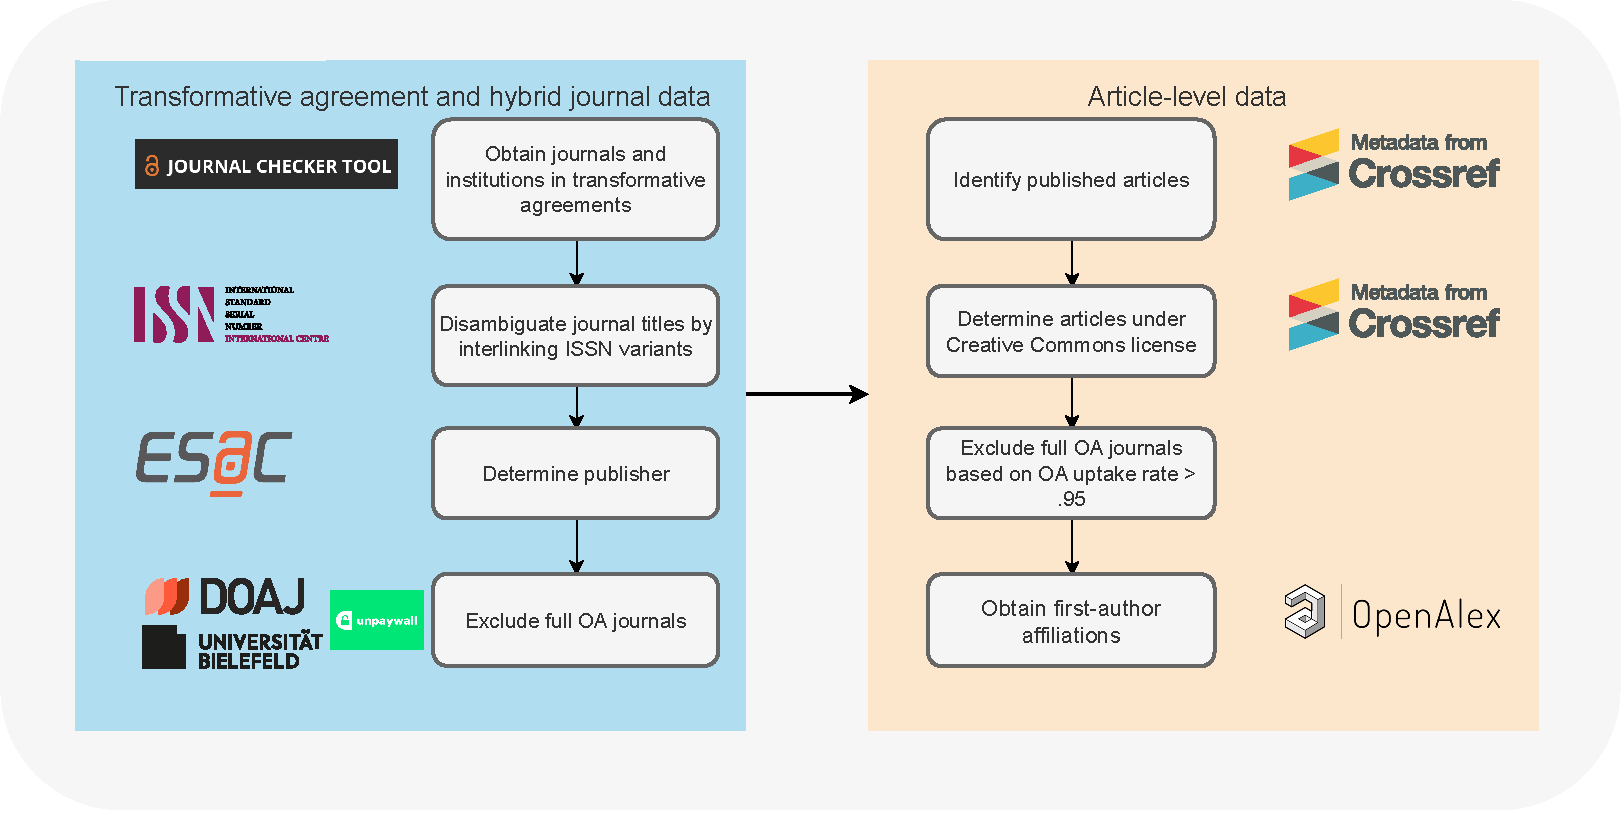
\includegraphics[width=0.99\linewidth,]{data_collection_workflow} 

}

\caption{Data collection workflow}\label{fig:data_workflow}
\end{figure}

\hypertarget{transformative-agreement-and-hybrid-journal-data}{%
\subsection{Transformative agreement and hybrid journal
data}\label{transformative-agreement-and-hybrid-journal-data}}

Data gathering started with obtaining journals included in
transformative agreements from the publicly available Transformative
Agreement Data dump\footnote{\url{https://journalcheckertool.org/transformative-agreements/}}
used by the cOAlition S Journal Checker Tool.\footnote{\url{https://www.coalition-s.org/blog/enabling-accurate-results-within-the-journal-checker-tool/}}
The dump consists of multiple online Google spreadsheets where each data
file represents one agreement listed in the ESAC Transformative
Agreement Registry.\footnote{\url{https://esac-initiative.org/about/transformative-agreements/agreement-registry/}}
From the retrieved spreadsheet files, journals and institutions involved
per agreement were obtained.

A limitation of using the Journal Checker Tool and its underlying
publicly available data dump to study the development of transformative
agreements over time is that expired transformative agreements are
constantly removed. To address this, four different snapshots were
safeguarded and combined for this study: self-archived versions from
July 2021, July 2022, and May 2023, as well as the most current dump
downloaded on 11 December 2023. This ensured that transformative
agreements, which ended from 2021 onwards, were included, representing
the majority of transformative agreements. Overall, the four combined
Transformative Agreement Data dumps used in this study contained 729 of
869 agreements listed in the ESAC registry by December 2023.

The Transformative Agreement Data dumps link agreements to journals
represented by journal names and the ISSN. After mapping ISSN variants
to the corresponding linking ISSN (ISSN-L), as provided by the ISSN
International Centre, journals were associated with publishers using the
ESAC ID, a unique identifier for transformative agreements in the ESAC
Transformative Agreement Registry. Furthermore, journal subjects
according to the All Science Journal Classification (ASJC) were added
from the Scopus journal source list as of August 2023.

Because transformative agreements can include both fully open access and
hybrid journals, the data were complemented with information about a
journal's open access status using multiple sources: the Directory of
Open Access Journals (DOAJ) downloaded on 12 December 2023\footnote{\url{https://doaj.org/csv}},
OpenAlex (November 2023) and the Bielefeld list of GOLD OA journals
(Bruns et al., 2022). As shown in Figure \ref{fig:method_fig}A,
combining different data sources considerably extended journal matching.
In total, 3,439 full open access journals were excluded based on ISSN
matching. The overlap between the three data sources was 72\%. The Gold
OA journals dataset alone added 176 journals, while the DOAJ comprised
10 fully open access journals not listed in either of the other two
sources. These fully open access journals were launched in 2022.

\hypertarget{article-and-author-metadata}{%
\subsection{Article and author
metadata}\label{article-and-author-metadata}}

After identifying hybrid journals included in transformative agreements,
article metadata were retrieved from the Crossref November 2023 database
snapshot for the five-year period from 2018 to 2022, according to the
issued date, representing the earliest known publication date. Because
Crossref metadata lacked information to distinguish between original
research articles, including reviews, and other types of journal
content, which are often not covered by transformative agreements
(Borrego et al., 2021), only articles published in regular issues
indicated by non-numeric pagination were included. Furthermore, paratext
recognition was applied to exclude non-scholarly journal content such as
table of contents.

Open access articles in hybrid journals were identified using the
Creative Commons (CC) license information in Crossref metadata. License
information relative to the ``accepted manuscript (AM)'' version was not
considered. Crossref was used for open access identification because
transformative agreement workflows generally require publishers to
deliver CC license information to this DOI registration agency (Geschuhn
\& Stone, 2017).

Comparing Crossref license coverage with OpenAlex, which re-uses open
access evidence from Unpaywall, a widely used open access discovery
service that also parses journal websites for open content licenses
(Piwowar et al., 2018), highlighted ongoing challenges in identifying
hybrid open access (Butler et al., 2023; Jahn et al., 2022;
Martín-Martín et al., 2018; Zhang et al., 2022). For the purpose of this
study, 742,369 articles under CC license were retrieved using Crossref,
while 950,260 articles were tagged as ``hybrid'' according to the
OpenAlex November 2023 release, which was used throughout this study.
The largest differences concerned articles published between 2018 and
2020. With regard to the publication year 2022, however, Crossref and
OpenAlex open access numbers differ only slightly (249,511 records using
Crossref vs.~255,344 in OpenAlex). Notable differences could be observed
among some publishers that presumably did not provide CC license
information to Crossref, including AIP Publishing, the American
Physiological Society, Emerald, and the Royal Society. Crossref license
metadata was more complete with regard to the articles published by
Wiley and the American Chemical Society. Finally, inconsistent open
access status information in previous OpenAlex versions was observed
(Jahn et al., 2023). After reporting this to OpenAlex, fixing this issue
was still ongoing according to the release notes, which might also
explain part of the discrepancy.

After retrieving the article metadata, the publication volume, including
open access, was calculated for each journal. To improve the
identification of hybrid journals, journals with an open access
proportion above 95\% were excluded. This step allowed removing
additional 241 fully open access journals.

Affiliation metadata about corresponding authors are crucial for the
planning and evaluation of transformative agreements because they are
considered responsible for arranging open access publication (Borrego et
al., 2021; Geschuhn \& Stone, 2017; Schimmer et al., 2015). For this
study, country and institutional affiliations were retrieved from
OpenAlex. However, because corresponding author affiliation was only
available for 54\% of the investigated articles in OpenAlex, this study
focused on first authors and their affiliations instead; approximately
90\% of the investigated articles had first author affiliation metadata
in OpenAlex, which is a much larger proportion than previoulsy reported
for the October 2022 snapshot (Zhang et al., 2024). First authors
typically contribute the most to a paper and are often considered being
lead authors (Larivière et al., 2016). Related studies also assumed
first authors as a proxy to examine open access payments and
transformative agreements (Haucap et al., 2021; Shu \& Larivière, 2023;
Zhang et al., 2022).

To estimate the impact of transformative agreements on hybrid open
access, participating institutions from the Transformative Agreement
Data dump, which the cOAlition S crowd-sourced from agreement documents
and consortia, were matched with the first author affiliations recorded
by OpenAlex using the ROR-ID. Matching also considered the duration of
agreements according to the ESAC registry. Upon inspection,
Transformative Agreement Data did not comprehensively cover associated
institutions, such as university hospitals or institutes of large
research organisations such as the Max Planck Society. To improve the
matching, Transformative Agreement Data were automatically enriched with
associated organisations using OpenAlex's institution entity data.

The so compiled data set consists of 8,922,146 articles published in
12,857 hybrid journals between 2018 and 2022 (see Figure
\ref{fig:method_fig}B). Hybrid journals in transformative agreements
represented 40\% of the total global output over the same time period,
according to Crossref, while fully open access journals recorded 35\%.

\begin{figure}[ht!]

{\centering 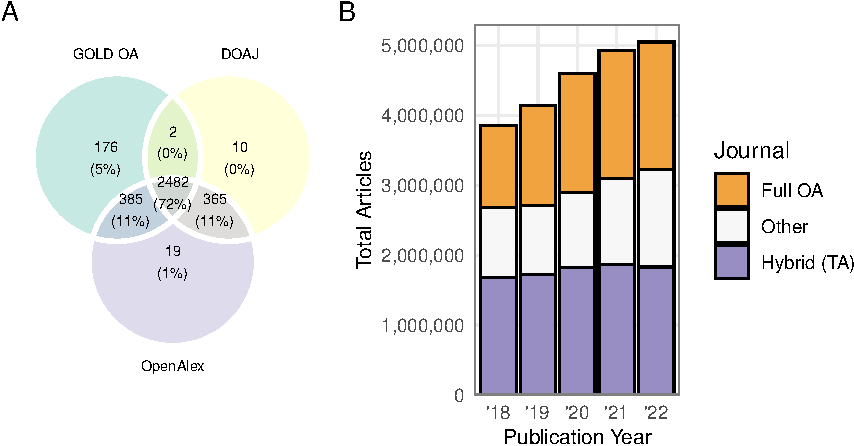
\includegraphics[width=0.99\linewidth,]{fig/method_fig-1} 

}

\caption{Initial data characteristics. (A) Full open access journals included in transformative agreements by evidence source Directory of Open Access Journals (DOAJ), OpenAlex and the Bielefeld GOLD OA list. (B) Number of articles in Crossref by journal types. The blue bars show the overall article volume of hybrid journals in transformative agreements, which were initially included in the study, in comparision with full open access journals according to OpenAlex. The remainder represents subscription-based journals not covered by transformative agreements.}\label{fig:method_fig}
\end{figure}

\hypertarget{data-analysis}{%
\subsection{Data analysis}\label{data-analysis}}

Throughout this mostly automated data gathering and analysis process,
Tidyverse tools (Wickham et al., 2019) for the R programming language (R
Core Team, 2020) were used. The resulting data are openly available
through an R data package, hoaddata (Jahn, 2023). Following Marwick et
al. (2018), hoaddata contains not only the datasets used in the data
analysis. It also includes code used to compile the data by connecting
it to the cloud-based Google Big Query data warehouse, where scholarly
big data from Crossref, OpenAlex and Unpaywall were imported, using
bigrquery (Wickham \& Bryan, 2023). To increase computational
reproducibility, data aggregation through hoaddata was automatically
carried out using GitHub Actions, a continuous integration service.

\hypertarget{results}{%
\section{Results}\label{results}}

\hypertarget{overview}{%
\subsection{Overview}\label{overview}}

Between 2018 and 2022, 11,189 out of 12,857 hybrid journals in
transformative agreements published at least one open access article
under a Creative Commons license. During this period, these hybrid
journals provided open access to 742,369 out of 8,146,958 articles,
representing a five-year open access proportion of 9.1\%. Authors who
could make use of transformative agreements at the time of publication
contributed 328,957 open access articles. Overall, 394 transformative
agreements recorded at least one open access article from an eligible
institution.

\begin{figure}[ht!]

{\centering 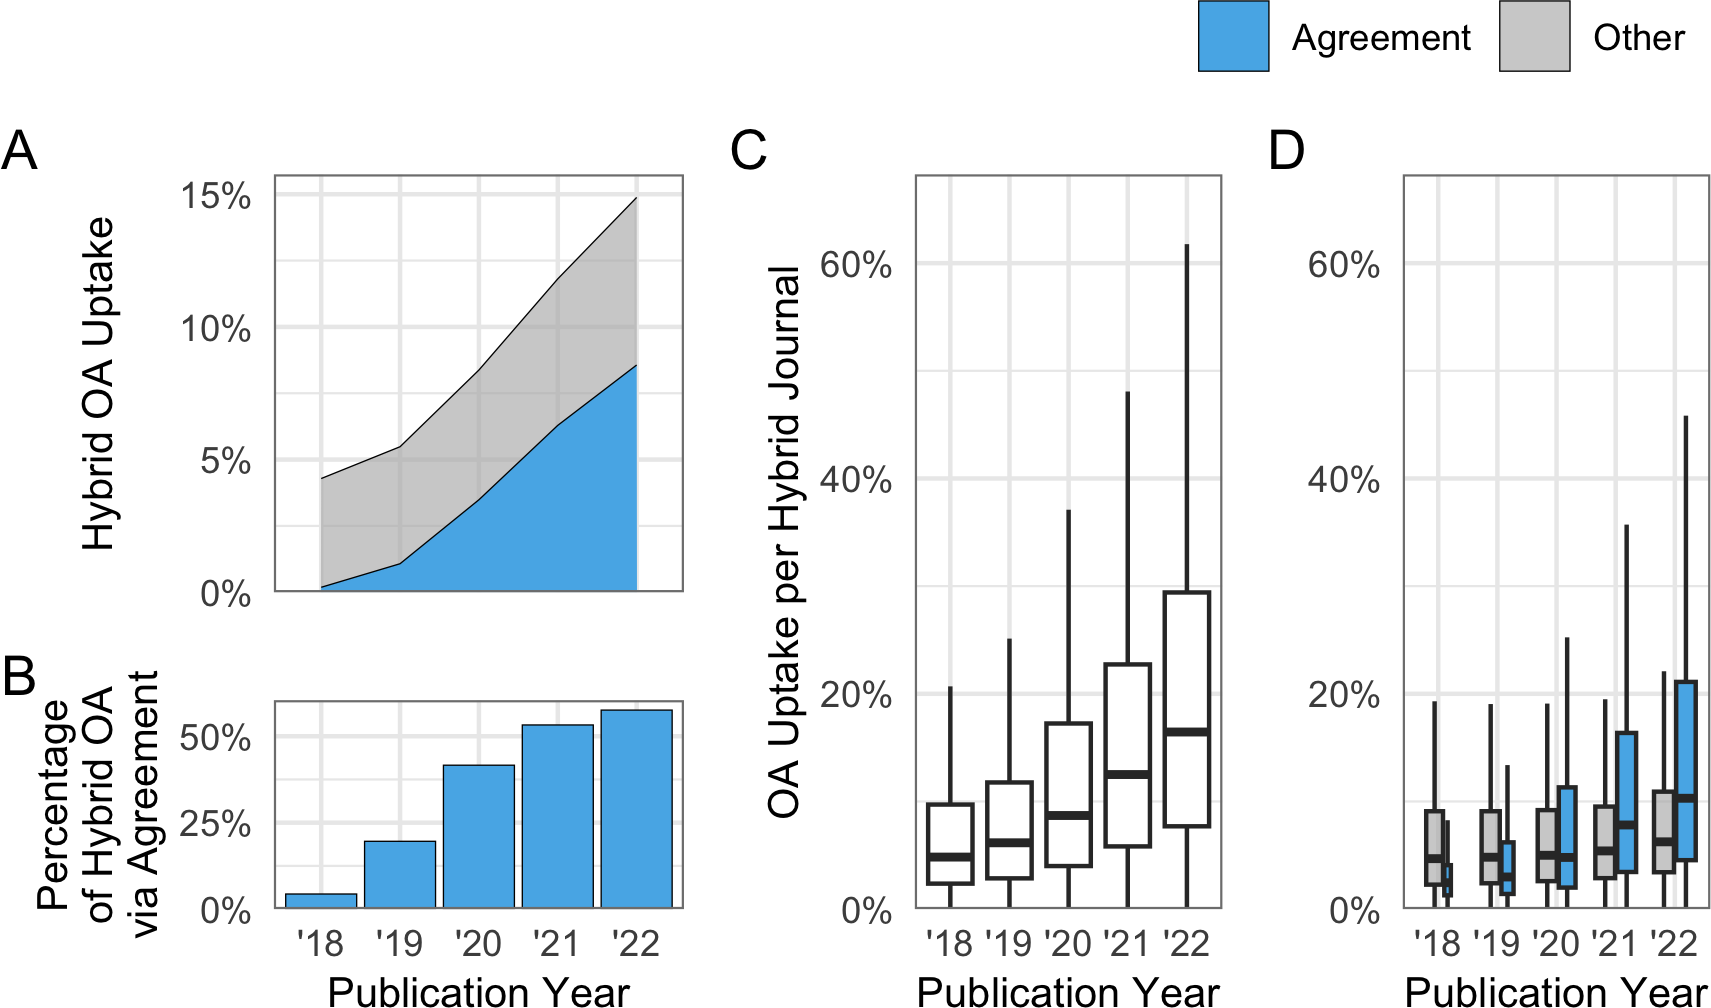
\includegraphics[width=0.99\linewidth,]{fig/results_overview-1} 

}

\caption{Relative growth of open access in hybrid journals in transformative agreements between 2018 and 2022 per publication year. The blue areas represent open access through transformative agreements, the grey areas depict open access articles where no link to an agreement could be established. (A) Proportion of open access articles in hybrid journals per year. (B) Percentage of hybrid open access via agreements per year. Boxplots show the proportion of open access articles by individual hybrid journals (C) and individual open access uptake rates by individual hybrid journals and open access funding (D) per publication year. The individual outliers are not shown. Note that data on transformative agreements ending before June 2021 were not available for this study.}\label{fig:results_overview}
\end{figure}

Figure \ref{fig:results_overview}A shows a moderate growth in the
proportion of open access articles in hybrid journals, comparing the
overall open access uptake and the impact of transformative agreements
on this trend. Over the five-years period from 2018 to 2022, open access
increased from 4.3\% (n = 65,486) to 15\% (n = 249,511). Simultaneously,
the total article volume of the investigated journals rose from
1,528,051 in 2018 to 1,676,928 in 2022.

Figure \ref{fig:results_overview}B highlights that the majority of
hybrid open access was made available through transformative agreements
in 2021 and 2022, contributing 58\% of the total open access article
volume in 2022. However, there was also a notable increase in open
access provision through other means, presumably publication fees being
not invoiced through transformative agreements, from 4.1\% (n = 62,625)
in 2018 to 6.3\% (n = 105,896) in 2022.

Figure \ref{fig:results_overview}C depicts the substantial variations
among the hybrid journals included in transformative agreements in terms
of open access uptake. Although the median generally follows the trend
shown in Figure \ref{fig:results_overview}A, the farther stretch of
upper quartiles and whiskers over the years illustrates that an
increasing number of journals published an above-average proportion of
open access articles. In 2022, 25\% of hybrid journals (n = 2,576) had
an open access uptake of 29\%, and 6.6\% of journals (n = 744) provided
the majority of their articles under a Creative Commons license in the
same year. On average, these journals were smaller (M = 75, SD = 186)
than those with an open access share below 50\% (M = 164, SD = 347).

When comparing the impact of open access through transformative
agreements across journals, it shows that for many journals, these
agreements substantially contributed to the growth of open access over
the years (Figure \ref{fig:results_overview}D). Despite the rise in
transformative agreements, it is worth noting that other means of
publishing open access remained common across the investigated hybrid
journals. In total, 9,153 journals published open access articles from
authors affiliated with institutions without transformative agreements
in place, while 8,780 journals published at least one open access
article through a transformative agreement in the same year.

\hypertarget{publishing-market}{%
\subsection{Publishing market}\label{publishing-market}}

Analysing hybrid open access across publishers between 2018 and 2022
reveals a large market concentration. Although 48 publishers offered
transformative agreements, the three commercial publishers Elsevier,
Springer Nature, and Wiley, accounted for 49\% of the total article
volume published (see Table \ref{tab:publisher_league_table}). Together,
they published 500,878 or 66\% of the open access articles in hybrid
journals. Elsevier, Springer Nature, and Wiley made 243,891 articles
open access in hybrid journals through transformative agreements,
resulting in an even larger market share of 74\%.

\begin{table}[H]

\caption{\label{tab:publisher_league_table}Hybrid open access through transformative agreements market shares 2018-2022}
\centering
\begin{tabular}[t]{lrlrlrlrl}
\toprule
\multicolumn{1}{c}{ } & \multicolumn{2}{c}{Hybrid journals} & \multicolumn{2}{c}{Articles} & \multicolumn{2}{c}{OA articles} & \multicolumn{2}{c}{TA OA articles} \\
\cmidrule(l{3pt}r{3pt}){2-3} \cmidrule(l{3pt}r{3pt}){4-5} \cmidrule(l{3pt}r{3pt}){6-7} \cmidrule(l{3pt}r{3pt}){8-9}
Publisher & Total & \% & Total & \% & Total & \% & Total & \%\\
\midrule
Elsevier & 1,936 & 17 & 2,770,826 & 33.8 & 172,723 & 22.9 & 60,440 & 18.3\\
Springer Nature & 2,274 & 20 & 1,330,430 & 16.2 & 175,432 & 23.3 & 100,008 & 30.3\\
Wiley & 1,410 & 12.4 & 1,043,052 & 12.7 & 152,723 & 20.3 & 83,443 & 25.3\\
Other & 5,767 & 50.6 & 3,061,337 & 37.3 & 252,523 & 33.5 & 86,294 & 26.1\\
\bottomrule
\end{tabular}
\end{table}

However, there are notable differences between the three large
publishers. Although Elsevier published the largest volume of articles
(n = 2,770,826, 34\%), it recorded a comparably low number of open
access articles, including those that are associated with transformative
agreements. In contrast, Springer Nature and Wiley provided open access
to a larger proportion of their articles (13\% of Springer Nature
articles and 15\% of Wiley articles were open access), leading to higher
open access market share (23\% Springer Nature resp. 23\% Wiley). This
difference between Elsevier on the one hand and Springer Nature and
Wiley on the other can be attributed to transformative agreements, as
the latter made the majority of their open access articles available
through such deals (Springer Nature 57\% resp. Wiley 55\%).

Figure \ref{fig:publisher_figure} takes a closer look into the growth of
hybrid open access across publishers by year, with a focus on open
access enabled by transformative agreements. Although all publishers
show a general long-term trend towards transformative agreements, Figure
\ref{fig:publisher_figure}A and B indicate that Wiley experienced a
substantial increase in its open access share from 5.9\% (n = 11,628) in
2018 to 26\% (n = 53,503) in 2022, representing a 4.5-fold increase. In
contrast, Elsevier's hybrid journals demonstrated a more modest
increase, from 3.3\% (n = 16,872) in 2018 to 10\% (n = 60,821) in 2022,
which is a relatively low open access share compared to the general
trend. In 2018, Springer Nature had the largest open access proportion
among the three publishers of 8.4\% (n = 19,701), but experienced a
relatively slower growth, resulting in 18\% (n = 52,616) of articles
being open access in Springer Nature hybrid journals in 2022.

\begin{figure}[ht!]

{\centering 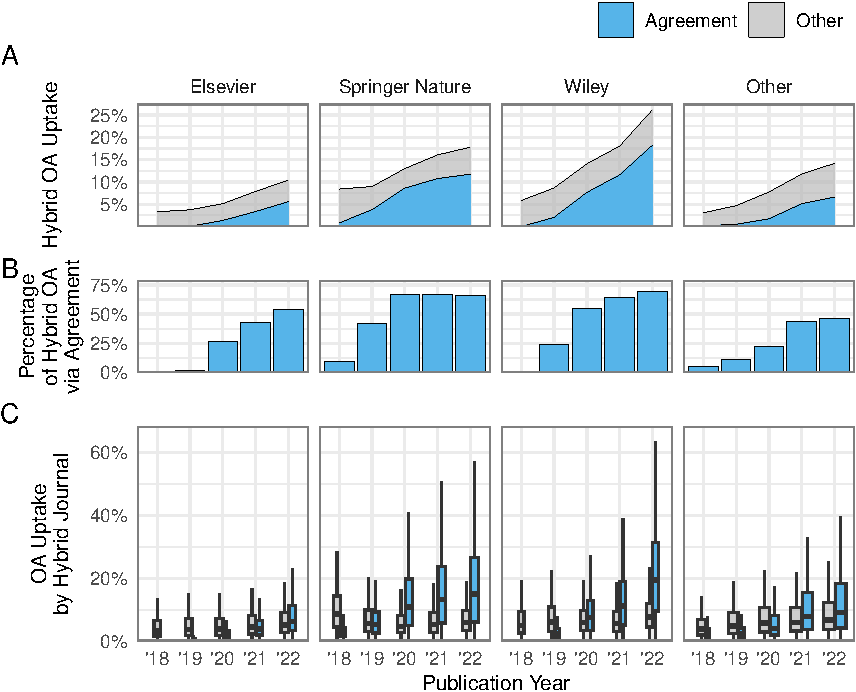
\includegraphics[width=0.99\linewidth,]{fig/publisher_figure-1} 

}

\caption{Developement of open access in hybrid journals included in transformative agreements between 2018 and 2022 by publishers. The blue areas represent open access through transformative agreements, the grey areas depict open access articles where no link to an agreement could be established. (A) Proportion of open access articles in hybrid journals per year and publisher. (B) Percentage of hybrid open access via agreements per year and publisher. Boxplots (C) show individual open access uptake rates by individual hybrid journals and open access funding per publication year and publisher. The individual outliers are not shown. Note that data on transformative agreements ending before June 2021 were not available for this study.}\label{fig:publisher_figure}
\end{figure}

The varying degrees of adoption of open access across the three major
publishers can be attributed to distinct approaches to transformative
agreements. Springer Nature, for example, started offering open access
agreements for its hybrid journal portfolio to selected consortia such
as the Max Planck Society, the Swedish Bibsam Consortium and the Finnish
FinELib consortium in 2015 under the name Springer Compact\footnote{\url{https://web.archive.org/web/20180414062853id_/http://www.liber2015.org.uk/wp-content/uploads/2015/03/Springer-Compact.pdf}}.
Prior to this, Springer had some pilot agreements with a small number of
institutions, including the University of Göttingen (Schmidt \& Shearer,
2012). However, the Springer Compact agreements were not included in the
data as they concluded before the start of the transformative agreement
data collection in June 2021. Nonetheless, the results demonstrate the
importance of agreements for Springer Nature's hybrid open access
business over the past five years (Figure 2B). In 2022, 66\% (n =
34,725) of open access in Springer Nature hybrid journals was enabled
through transformative agreements. In the same year, 70\% (n = 37,316)
of Wiley's open access articles could be linked to transformative
agreements in 2022. By contrast, Elsevier published fewer than half of
its open access articles through transformative agreements (n = 32,627;
54\%).

The increasing trend towards transformative agreements can also be
observed at the journal-level (Figure \ref{fig:publisher_figure}C).
While no substantial differences between open access enabled through
transformative agreements and other revenue sources could be seen across
Elsevier's portfolio, the distribution of open access across Springer
Nature and Wiley hybrid journals indicates that the growth is not
limited to a few journals but extends across the portfolio. In
particular, Wiley's upper quantile, which represents the top 25\% of
journals in terms of the proportion of open access articles from
transformative agreements, increased markedly from 13\% in 2020 to 31\%
in 2022. Simultaneously, the median proportion increased from 7.5\% to
19\%. It is interesting to note that a small but increasing number of
journals from these two publishers provide open access to the majority
of articles through transformative agreements. Wiley recorded 68 and
Springer Nature 102 hybrid journals with an open access share above
50\%, which could be attributed solely to transformative agreements.
Upon inspection, these journals were mainly society or local language
journals with small annual article volumes.

\hypertarget{journal-subjects}{%
\subsection{Journal subjects}\label{journal-subjects}}

Table \ref{tab:subject_summary_table} presents a high-level overview of
hybrid open access by AJCS subject area using fractionalised counting to
account for journals belonging to more than one category. Between 2018
and 2022, most hybrid journals with at least one open access article
could be attributed to the Social Sciences category, which also includes
Arts and Humanities. However, these journals published the fewest number
of articles, whereas Physical Sciences journals recorded the most
articles, followed by Health Sciences and Life Sciences. In terms of
open access, Physical Sciences journals accounted for more than
one-third of the articles published in the five-year period, followed by
Health Sciences, Social Sciences and Life Sciences.

\begin{table}[H]

\caption{\label{tab:subject_summary_table}Hybrid open access through transformative agreements by journal subject 2018-2022}
\centering
\begin{tabular}[t]{lrlrlrlrl}
\toprule
\multicolumn{1}{c}{ } & \multicolumn{2}{c}{Hybrid journals} & \multicolumn{2}{c}{Articles} & \multicolumn{2}{c}{OA articles} & \multicolumn{2}{c}{TA OA articles} \\
\cmidrule(l{3pt}r{3pt}){2-3} \cmidrule(l{3pt}r{3pt}){4-5} \cmidrule(l{3pt}r{3pt}){6-7} \cmidrule(l{3pt}r{3pt}){8-9}
Journal subject & Total & \% & Total & \% & Total & \% & Total & \%\\
\midrule
Health Sciences & 2,342 & 22.5 & 1,998,045 & 28 & 199,265 & 27.7 & 81,913 & 25.7\\
Life Sciences & 1,399 & 13.4 & 1,080,346 & 15.1 & 133,526 & 18.6 & 48,570 & 15.2\\
Physical Sciences & 2,693 & 25.9 & 3,111,711 & 43.6 & 247,515 & 34.4 & 110,933 & 34.8\\
Social Sciences & 3,967 & 38.1 & 953,084 & 13.3 & 138,388 & 19.3 & 77,496 & 24.3\\
\bottomrule
\end{tabular}
\end{table}

Figure \ref{fig:subject_panel} presents the relative growth of hybrid
open access by subject area between 2018 and 2022. In particular, Social
Sciences including Arts and Humanties journals accounted for the
strongest growth in the five-years period from 6.4\% (n = 8,361) to 23\%
(n = 51,938), followed by the Life Sciences from 7.6\% (n = 15,003) to
18\% (n = 39,494) , Health Sciences from 5.3\% (n = 18,279) to 16\% (n =
63,089) and Physical Sciences from 4.5\% (n = 22,364) to 12\% (n =
85,428). Growth in Social Sciences category can be largely attributed to
transformative agreements. In 2022, two-thirds of open access articles
(67\%, n = 34,759) were published by the first authors affiliated with
participating institutions (see \ref{fig:subject_panel}B).

\begin{figure}[ht!]

{\centering 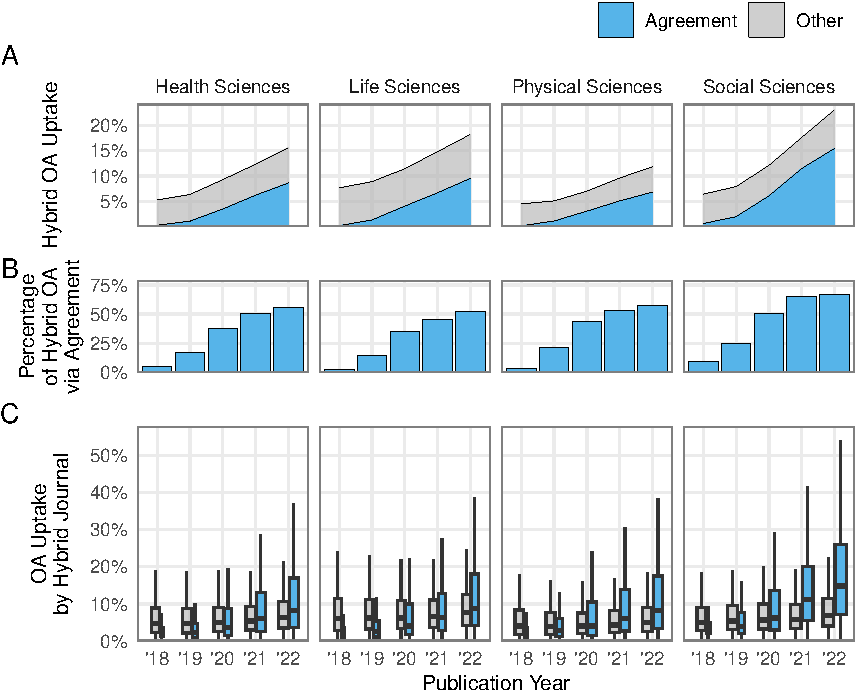
\includegraphics[width=0.99\linewidth,]{fig/subject_panel-1} 

}

\caption{Developement of open access in hybrid journals in transformative agreements between 2018 and 2022 by AJCS subject area. The blue areas represent open access through transformative agreements, the grey areas depict open access articles where no link to an agreement could be established. (A) Proportion of open access articles in hybrid journals per year and publisher. (B) Percentage of hybrid open access via agreements per year and publisher. Boxplots (C) show individual open access uptake rates by individual hybrid journals and open access funding per publication year and publisher. The individual outliers are not shown. Note that data on transformative agreements ending before June 2021 were not available for this study.}\label{fig:subject_panel}
\end{figure}

Figure \ref{fig:subject_panel}C shows that this trend was consistent
across hybrid journals belonging to the ASJC Social Sciences category.
In 2022, 25\% of Social Sciences journals provided open access to at
least every fourth article exclusively through transformative
agreements. However, hybrid open access through transformative
agreements played a comparably lesser role in Life Sciences and Health
Sciences. In these two subject areas, only about half of the open access
articles can be linked to these agreements, both overall and on a median
average across journals. In contrast, the majority of Physical Science
journals show an increase of open access through transformative
agreements compared to other options to publish open access in hybrid
journals.

\hypertarget{comparing-countries}{%
\subsection{Comparing countries}\label{comparing-countries}}

Between 2018 and 2022, high-income countries almost exclusively
dominated hybrid open access publishing through transformative
agreements. During this period, first authors affiliated with
institutions from Organisation for Economic Co-operation and Development
(OECD) member countries published 602,050 open access articles in hybrid
journals, representing 81\% of the investigated open access articles.
This disparity between OECD nations and other countries becomes even
more evident when considering open access through transformative
agreements, as 310,712 of 328,957, or 94\% of open access articles were
associated with such agreements.

Figure \ref{fig:country_patch}A shows the development of hybrid open
access publishing by country, comparing the OECD area with the BRICS, an
intergovernmental organisation, which comprised Brazil, Russia, India,
China, and South Africa as of 2022. The residual category ``Other''
includes the remaining countries. Full counting was applied to account
for multiple country affiliations (Hottenrott et al., 2021). From 2018
to 2022, the proportion of open access in hybrid journals increased from
6.1\% in 2018 to 26\% in 2022. In contrast, BRICS recorded a low uptake,
moderately growing from 1.6\% in 2018 to 3.7\% in 2022.

Despite the rise of open access across OECD countries, the overall
publication output decreased sharply, dropping to 786,903 in 2022 after
peaking 892,197 articles in 2020. In stark contrast, the number of
articles published in hybrid journals by first authors affiliated with
institutions from BRICS countries increased steadily over the years,
more than doubling from 356,632 in 2018 to 786,903 in 2022. Upon closer
examination, this trend can be observed across all of the three largest
publishers, although the shift towards BRICS is particularly evident in
Elsevier's hybrid journal portfolio, particularly with regard to
articles published in Physical Sciences journals. While OECD publication
output in Elsevier's Physical Sciences journals declined from 112,822
articles in 2018 to 103,766 in 2022, BRICS output increased from 104,654
to 171,713 in the same five-year period. Furthermore, OECD publication
output in Health Sciences and Life Sciences journals stagnated after
peaking in 2020.

\begin{figure}[ht!]

{\centering 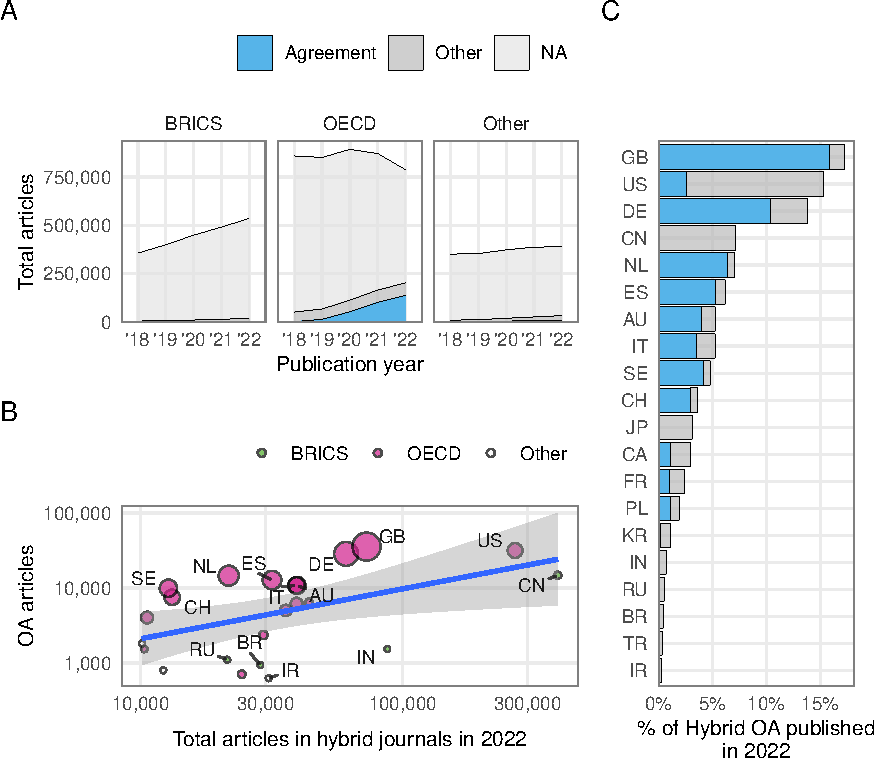
\includegraphics[width=0.99\linewidth,]{fig/country_patch-1} 

}

\caption{Development of hybrid open access publishing by country. (A) presents the number of articles published in hybrid journals included in transformative agreement, distinguishing between BRICS as of 20222, OECD and other countries. (B) Scatterplot contrasting total articles with open access article volume in 2022, by country. Point size represents the number of articles enabled through transformative agreements. (C) Hybrid open access market share in 2022 by country. In (A) and (C), the blue areas represent open access through transformative agreements, the grey areas depict open access articles where no link to an agreement could be established. Country names are represented as ISO two-letter country codes.}\label{fig:country_patch}
\end{figure}

To illustrate the situation in 2022, Figure \ref{fig:country_patch}B
compares the total publication output with the number of open access
articles. With 391,530 articles, China was the most productive country,
followed by the United States (n = 268,965) and India (n = 87,428). In
contrast, Western and Northern European countries published a
considerably high number of open access articles. Particularly,
Scandinavian countries, the Netherlands and Austria recorded
above-average open access shares, as indicated by the linear trend line.
As shown in Figure \ref{fig:country_patch}C, transformative agreements
contributed to these market positions. Interestingly, the United States
had a notable open access market share of 15\%, although transformative
agreements contributed to a lesser extent. Similarly, China's open
access market share of 7.2\% in 2022 was comparable to that of the
Netherlands, which was 7.1\%.

Figure \ref{fig:country_top_20_plot} illustrates the development of
hybrid open access from 2018 to 2022, highlighting the top 20 most
productive countries in terms of articles published in hybrid journals
that were included in transformative agreements over the five-year
period. Notably, the Netherlands (27\%), Sweden (24\%), Poland (17\%)
and Great Britain (17\%) exhibited a relatively high level of uptake in
2018 which continued to increase in the following years. In 2022, Sweden
had the highest proportion of open access relative to its publication
output (78\%), followed by the Netherlands (67\%) and Switzerland
(57\%), with these countries benefiting from transformative agreements.
In Germany, however, hybrid open access only began to increase from 2019
onwards after the successful negotiation of nationwide agreements with
Wiley (July 2019) and Springer Nature (January 2020). Prior to this,
only a few organisations had agreements in place, for example, the Max
Planck Society with Springer Compact.

\begin{figure}[ht!]

{\centering 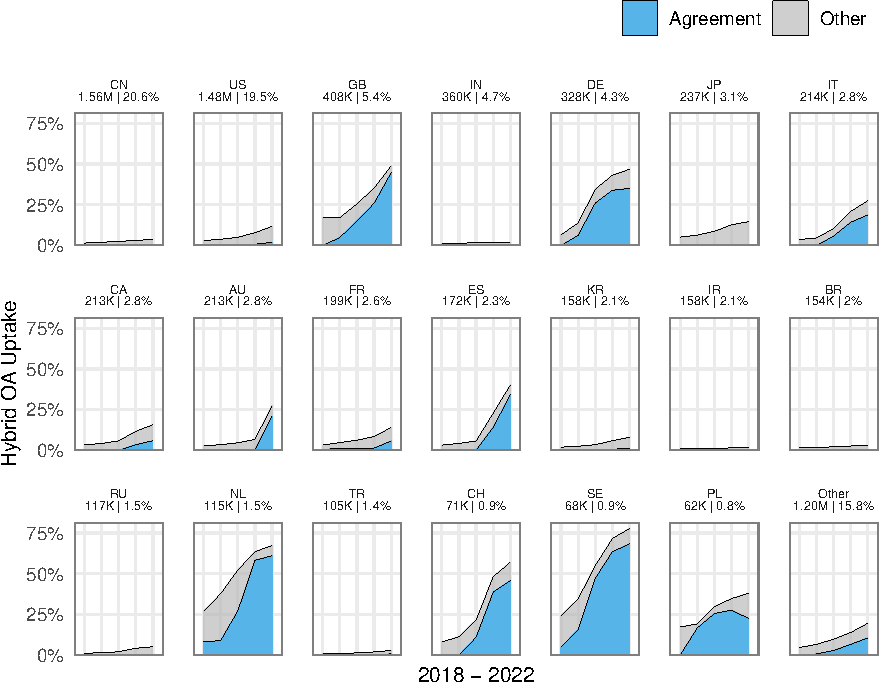
\includegraphics[width=0.99\linewidth,]{fig/country_top_20_plot-1} 

}

\caption{Development of open access in hybrid journals in transformative agreements between 2018 and 2022, by the Top 20 most productive countries in terms of total articles published in the five-years period. Blue areas represent open access through transformative agreements, the grey areas depict open access articles where no link to an agreement could be established. Country names are represented as ISO two-letter country codes. Facet subheadings show the total number of articles and corresponding market share.}\label{fig:country_top_20_plot}
\end{figure}

Since 2021, there has been a general trend towards hybrid open access
among many high-income countries, driven primarily by transformative
agreements. However, the proliferation of transformative agreements
differed across these countries. Additionally, publication limits or
eligibility criteria for institutions and article types may explain why
even countries with widespread agreement implementation such as Sweden
or the Netherlands did not achieve 100\% hybrid open access.
Interestingly, in Japan and the United States, options other than
transformative agreements were the main drivers for the increase in
hybrid open access. Once again, the graph highlights countries with low
hybrid open access, particularly non-OECD countries, where only a few or
no agreements were in place.

\hypertarget{discussion}{%
\section{Discussion}\label{discussion}}

The primary aim of this study was to assess the uptake of open access in
hybrid journals included in transformative agreements, which were
introduced as a temporal means to support the transition of
subscription-based academic publishing to full open access. This study
presents a novel approach based on open data, which leverages metadata
on over 700 agreements and nine million journal articles to estimate the
extent to which transformation agreements contribute to the transition
of this journal business model. The results highlight a strong growth in
open access between 2018 and 2022, driven by an increasing number of
institutions that had transformative agreements in place. However, the
majority of research literature published in hybrid journals in this
five-year period remained behind publisher paywalls. Growth in the
adoption of open access in hybrid journals, in particular through
transformative agreements, can be largely attributed to three large
commercial publishers -- Elsevier, Springer Nature, and Wiley -- but
varies substantially across journals, publishers, disciplines, and
country affiliations. Despite the limitations of the data, the findings
indicate that the current level of implementation of transformative
agreements is insufficient to bring about a large-scale transition to
fully open access.

A key finding of this analysis is that transformative agreements
maintain market concentration. Specifically, the three largest
commercial publishers Elsevier, Springer Nature, and Wiley dominate,
particularly with regard to open access provided through transformative
agreements. Together, the three publishers accounted for three-fourths
of open access articles through transformative agreements, while
recording less than half of the total publication volume published
between 2018 and 2022. This observation aligns with previous research on
shifts in the publishing market following the introduction of funding
opportunities for hybrid open access (Butler et al., 2023; Jahn \&
Tullney, 2016; Shu \& Larivière, 2023). Additionally, the results
confirm previously observed variations by publisher, with Elsevier
exhibiting a different development than Springer Nature and Wiley
(Butler et al., 2023; Jahn et al., 2022). However, it must be noted that
the focus of transformative agreements on publishers with large hybrid
journal portfolios is intentional (Campbell et al., 2022). Because of
transformative agreements with a few large publishers, national
consortia were able to substantially increase their country's annual
open access article volume (Bosman, Jonge, et al., 2021; Huang et al.,
2020; Pinhasi et al., 2021; Taubert et al., 2023; Wenaas, 2022).

Moreover, this study presents varying levels of open access uptake
through transformative agreements across journals, which can be
attributed to the alignment of authors' affiliations and the
availability of such agreements at their institutions. In line with
previous research findings (Butler et al., 2023; Jahn et al., 2022;
Wenaas, 2022), high uptake rates were observed across hybrid journals in
Social Sciences and Humanities. However, it is important to emphasise
that these hybrid journals do not encompass the entire field. For
example, Khanna et al. (2022) found that approximately 60\% of journals
utilizing the open-source publishing platform Open Journal Systems (OJS)
fall within the Social Sciences and Humanities. In these fields, the
majority of full open access journals are so-called ``Diamond OA
journals'', which do not charge publication fees (Bosman, Frantsvåg, et
al., 2021). Rather, this result can be more accurately attributed to the
substantial proportion of authors from high-income countries who publish
in these hybrid journals included in transformative agreements,
particularly when journals are of local relevance, such as by belonging
to national societies or regional research scope.

Surprisingly, the total publication output of high-income countries
belonging to the OECD in hybrid journals declined substantially after
peaking in 2020, whereas that of BRICS countries doubled from 2018 to
2022. Because the BRICS expansion can be exclusively attributed to
closed access articles, this development has the potential to hinder the
transition of academic journal publishing to full open access through
transformative agreements and demands discussion. In China, the country
with the highest volume of articles in hybrid journals, only limited
research funding to pay for open access is available, with expenditures
for open access publishing surpassing subscription costs (Shu \&
Larivière, 2023). Furthermore, the focus of Chinese authors on
established journals may contribute to this trend (Zhang et al., 2022).
Although China supports Plan S (Schiermeier, 2018), this is not
reflected in the data in terms of open access uptake in hybrid journals.
As highlighted by Koley \& Lala (2023), India faces similar challenges
in terms of the availablility of resources to pay for open access. At
the same time, access to research literature is a pressing issue, which
is addressed by the ``Indian one nation, one subscription'' policy
proposal. However, this policy focuses on centrally negotiated
subscriptions and does not entail open access.

But open access uptake also differs among OECD countries. In the United
States, for example, hybrid open access, including transformative
agreements, plays a lesser role than in some European countries. Between
2017 and 2021, hybrid open access contributed the least to openly
available federally funded research articles (Schares, 2023). While some
university consortia, such as the California Digital Library, have
signed transformative agreements, others have attempted to depart from
big deals and unbundle large journal portfolios to address cost
increases (Brainard, 2021; Schares, 2022). Despite the relatively low
penetration of transformative agreements in China and the United States
compared to Europe, 22\% of open access in hybrid journals in 2022
originates from these two countries, indicating the availability of
funding sources for publication fees.

This large-scale study provides the first empirical evidence of the
influence of transformative agreements on the transition of hybrid
journals to full open access. However, several limitations needs to be
acknowledged. From a data perspective, estimations of open access
through transformative agreements were established by linking first
author affiliations with publicly available agreement data from
cOAlition S, and not through invoicing data, which is usually not
shared. Moreover, this study is unable to account for the various types
of transformative agreements, particularly with regard to article types
and caps that limit the number of open access articles covered.
Furthermore, assessing the quality of the OpenAlex and Crossref data
used, particularly in terms of affiliations and article types, by
combining them with established bibliometric databases such as Scopus
and Web of Science was beyond the scope of this analysis (Visser et al.,
2021). Overall, the methodology is designed in such a way that the
results underestimate rather than overestimate the adoption of open
access through transformative agreements. In addition, the data used in
this study are openly available, along with the code used for this
analysis.

Additionally, it must be noted that the study period was significantly
impacted by the COVID-19 pandemic, which led to an unprecedented number
of publications and a reduction in international collaboration
(Aviv-Reuven \& Rosenfeld, 2021), which could explain the observed
contrasting developments in OECD and BRICS countries. However, even
before the pandemic, growth in publications in Europe was only due to
internationally co-authored journal articles (Kwiek, 2021). Likewise,
inflows from China to the United States and European countries already
declined by 2020 (Zhao et al., 2023). Furthermore, the study design did
not consider emerging publication practices such as preprints (Fraser et
al., 2021) and special issues (Hanson et al., 2023), which have grown
rapidly since 2020. Lastly, it should be emphasised that the study did
not address financial shifts between subscriptions spending and open
access payments while analysing hybrid open access through
transformative agreements due to a lack of data on expenditures.

This study allows for multiple strands of further research. One is to
complement this large-scale study with more specific evidence from
individual countries or subjects, particularly those with low hybrid
open access rates. Incorporating full open access and subscription-based
journals, as well as considering global trends in scholarly migration
and collaboration could also be promising. Financial studies could build
on the study design and include subscription and open access expenditure
to assess the cost-effectiveness of transformative agreements, in
particular whether transformative agreements can integrate the
substantial amounts of individual payments for publication fees (Butler
et al., 2023; Wenaas, 2022), as well as potential changes in authors'
behaviour following the introduction of these agreements (Schmal, 2024).

This study has practical implications for research funding and
libraries. Of primary concern should be the observed differences across
countries, particularly the relationship between economic development
and open access adoption. From a data perspective, the reporting of open
access funding, including transformative agreements, is not harmonised,
but often crowd-sourced from various sources. To improve the assessment
of transformative agreements, libraries and publishers need to
collaborate on standards and services to publicly share information
about respective journal portfolios, participating institutions and open
access invoicing.

In summary, this study provides empirical insights into the development
of hybrid open access following the introduction of transformative
agreements. These results are important for both researchers and
stakeholders engaged in negotiating and evaluating these agreements. The
presented approach relies on open data, which enables follow-up studies
and open access monitoring activities to further explore the role of
transformative agreements in transitioning academic publishing to full
open access.

\hypertarget{competing-interests}{%
\section{Competing interests}\label{competing-interests}}

The author declares no competing interests.

\hypertarget{funding-information}{%
\section{Funding information}\label{funding-information}}

This work was supported by the Deutsche Forschungsgemeinschaft (Grant
number 416115939).

\hypertarget{data-and-code-availability}{%
\section{Data and code availability}\label{data-and-code-availability}}

Source code analysis including data used is available on GitHub:
\url{https://github.com/njahn82/hoa_ta_effects}.

\hypertarget{references}{%
\section*{References}\label{references}}
\addcontentsline{toc}{section}{References}

\hypertarget{refs}{}
\begin{CSLReferences}
\leavevmode\vadjust pre{\hypertarget{ref-Aviv_Reuven_2021}{}}%
Aviv-Reuven, S., \& Rosenfeld, A. (2021). Publication patterns' changes
due to the COVID-19 pandemic: A longitudinal and short-term
scientometric analysis. \emph{Scientometrics}, \emph{126}(8),
6761--6784. \url{https://doi.org/10.1007/s11192-021-04059-x}

\leavevmode\vadjust pre{\hypertarget{ref-budapest}{}}%
Babini, D., Chan, L., Hagemann, M., Joseph, H., Kuchma, I., \& Suber, P.
(2022). \emph{{The Budapest Open Access Initiative-20th. Anniversary
recommendations (BOAI20)}}.
\url{https://www.budapestopenaccessinitiative.org/boai20/}

\leavevmode\vadjust pre{\hypertarget{ref-Bakker_2024}{}}%
Bakker, C., Langham-Putrow, A., \& Riegelman, A. (2024). Impact of
transformative agreements on publication patterns: An analysis based on
agreements from the ESAC registry. \emph{International Journal of
Librarianship}, \emph{8}(4), 67--96.
\url{https://doi.org/10.23974/ijol.2024.vol8.4.341}

\leavevmode\vadjust pre{\hypertarget{ref-Bergstrom_2014}{}}%
Bergstrom, T. C., Courant, P. N., McAfee, R. P., \& Williams, M. A.
(2014). Evaluating big deal journal bundles. \emph{Proceedings of the
National Academy of Sciences}, \emph{111}(26), 9425--9430.
\url{https://doi.org/10.1073/pnas.1403006111}

\leavevmode\vadjust pre{\hypertarget{ref-Bj_rk_2012}{}}%
Björk, B.-C. (2012). The hybrid model for open access publication of
scholarly articles: A failed experiment? \emph{Journal of the American
Society for Information Science and Technology}, \emph{63}(8),
1496--1504. \url{https://doi.org/10.1002/asi.22709}

\leavevmode\vadjust pre{\hypertarget{ref-Bj_rk_2017}{}}%
Björk, B.-C. (2017). Growth of hybrid open access, 2009--2016.
\emph{PeerJ}, \emph{5}, e3878. \url{https://doi.org/10.7717/peerj.3878}

\leavevmode\vadjust pre{\hypertarget{ref-BJ_RK_2014}{}}%
Björk, B.-C., \& Solomon, D. (2014). How research funders can finance
APCs in full OA and hybrid journals. \emph{Learned Publishing},
\emph{27}(2), 93--103. \url{https://doi.org/10.1087/20140203}

\leavevmode\vadjust pre{\hypertarget{ref-Borrego_2023}{}}%
Borrego, Á. (2023). Article processing charges for open access journal
publishing: A review. \emph{Learned Publishing}, \emph{36}(3), 359--378.
\url{https://doi.org/10.1002/leap.1558}

\leavevmode\vadjust pre{\hypertarget{ref-Borrego_2020}{}}%
Borrego, Á., Anglada, L., \& Abadal, E. (2021). Transformative
agreements: Do they pave the way to open access? \emph{Learned
Publishing}, \emph{34}(2), 216--232.
\url{https://doi.org/10.1002/leap.1347}

\leavevmode\vadjust pre{\hypertarget{ref-bosman_2021_4558704}{}}%
Bosman, J., Frantsvåg, J. E., Kramer, B., Langlais, P.-C., \& Proudman,
V. (2021). \emph{{OA Diamond Journals Study}. Part 1: findings}. Zenodo.
\url{https://doi.org/10.5281/zenodo.4558704}

\leavevmode\vadjust pre{\hypertarget{ref-Bosman_2021}{}}%
Bosman, J., Jonge, H. de, Kramer, B., \& Sondervan, J. (2021). Advancing
open access in the {Netherlands} after 2020: From quantity to quality.
\emph{Insights the UKSG Journal}, \emph{34}.
\url{https://doi.org/10.1629/uksg.545}

\leavevmode\vadjust pre{\hypertarget{ref-Brainard_2021}{}}%
Brainard, J. (2021). California universities and {Elsevier} make up, ink
big open-access deal. \emph{Science}.
\url{https://doi.org/10.1126/science.abi5505}

\leavevmode\vadjust pre{\hypertarget{ref-Brainard_2023}{}}%
Brainard, J. (2023). {`Transformative'} journals get booted for
switching to open access too slowly. \emph{Science}.
\url{https://doi.org/10.1126/science.adj3282}

\leavevmode\vadjust pre{\hypertarget{ref-goldoa}{}}%
Bruns, A., Cakir, Y., Kaya, S., \& Beidaghi, S. (2022).
\emph{{ISSN-Matching of Gold OA Journals (ISSN-GOLD-OA) 5.0}}. Bielefeld
University. \url{https://doi.org/10.4119/unibi/2961544}

\leavevmode\vadjust pre{\hypertarget{ref-Butler_2023}{}}%
Butler, L.-A., Matthias, L., Simard, M.-A., Mongeon, P., \& Haustein, S.
(2023). The oligopoly's shift to open access: How the big five academic
publishers profit from article processing charges. \emph{Quantitative
Science Studies}, 1--22. \url{https://doi.org/10.1162/qss_a_00272}

\leavevmode\vadjust pre{\hypertarget{ref-ifla}{}}%
Campbell, C., Dér, Á., Geschuhn, K., \& Valente, A. (2022). How are
transformative agreements transforming libraries? \emph{87th IFLA World
Library and Information Congress (WLIC) / 2022 in Dublin, Ireland}.
\url{https://repository.ifla.org/handle/123456789/1973}

\leavevmode\vadjust pre{\hypertarget{ref-Dallmeier_2010}{}}%
Dallmeier-Tiessen, S., Goerner, B., Darby, R., Hyppoelae, J.,
Igo-Kemenes, P., Kahn, D., Lambert, S., Lengenfelder, A., Leonard, C.,
Mele, S., Polydoratou, P., Ross, D., Ruiz-Perez, S., Schimmer, R.,
Swaisland, M., \& Stelt, W. van der. (2010). \emph{{Open Access
Publishing - Models and Attributes}}. The SOAP consortium.
\url{https://hdl.handle.net/11858/00-001M-0000-0013-838A-6}

\leavevmode\vadjust pre{\hypertarget{ref-Fraser_2021}{}}%
Fraser, N., Brierley, L., Dey, G., Polka, J. K., Pálfy, M., Nanni, F.,
\& Coates, J. A. (2021). The evolving role of preprints in the
dissemination of COVID-19 research and their impact on the science
communication landscape. \emph{PLOS Biology}, \emph{19}(4), e3000959.
\url{https://doi.org/10.1371/journal.pbio.3000959}

\leavevmode\vadjust pre{\hypertarget{ref-Fraser_2023}{}}%
Fraser, N., Hobert, A., Jahn, N., Mayr, P., \& Peters, I. (2023). No
deal: German researchers' publishing and citing behaviors after big deal
negotiations with {Elsevier}. \emph{Quantitative Science Studies},
\emph{4}(2), 325--352. \url{https://doi.org/10.1162/qss_a_00255}

\leavevmode\vadjust pre{\hypertarget{ref-Geschuhn_2017}{}}%
Geschuhn, K., \& Stone, G. (2017). It's the workflows, stupid! What is
required to make {`offsetting'} work for the open access transition.
\emph{Insights the {UKSG} Journal}, \emph{30}(3), 103--114.
\url{https://doi.org/10.1629/uksg.391}

\leavevmode\vadjust pre{\hypertarget{ref-hanson2023strain}{}}%
Hanson, M. A., Barreiro, P. G., Crosetto, P., \& Brockington, D. (2023).
\emph{The strain on scientific publishing}.
\url{https://arxiv.org/abs/2309.15884}

\leavevmode\vadjust pre{\hypertarget{ref-Haucap_2021}{}}%
Haucap, J., Moshgbar, N., \& Schmal, W. B. (2021). The impact of the
{German {``DEAL''}} on competition in the academic publishing market.
\emph{Managerial and Decision Economics}, \emph{42}(8), 2027--2049.
\url{https://doi.org/10.1002/mde.3493}

\leavevmode\vadjust pre{\hypertarget{ref-Hendricks_2020}{}}%
Hendricks, G., Tkaczyk, D., Lin, J., \& Feeney, P. (2020). Crossref: The
sustainable source of community-owned scholarly metadata.
\emph{Quantitative Science Studies}, \emph{1}(1), 414--427.
\url{https://doi.org/10.1162/qss_a_00022}

\leavevmode\vadjust pre{\hypertarget{ref-Hinchliffe_2019}{}}%
Hinchliffe, L. J. (2019). \emph{Transformative agreements: A primer}.
The Scholarly Kitchen.
\url{https://web.archive.org/web/20210128170342/https://scholarlykitchen.sspnet.org/2019/04/23/transformative-agreements/}

\leavevmode\vadjust pre{\hypertarget{ref-Hottenrott_2021}{}}%
Hottenrott, H., Rose, M. E., \& Lawson, C. (2021). The rise of multiple
institutional affiliations in academia. \emph{Journal of the Association
for Information Science and Technology}, \emph{72}(8), 1039--1058.
\url{https://doi.org/10.1002/asi.24472}

\leavevmode\vadjust pre{\hypertarget{ref-Huang_2020}{}}%
Huang, C.-K. (Karl), Neylon, C., Hosking, R., Montgomery, L., Wilson, K.
S., Ozaygen, A., \& Brookes-Kenworthy, C. (2020). Evaluating the impact
of open access policies on research institutions. \emph{{eLife}},
\emph{9}. \url{https://doi.org/10.7554/elife.57067}

\leavevmode\vadjust pre{\hypertarget{ref-hoaddata}{}}%
Jahn, N. (2023). \emph{{hoaddata}: Data about hybrid open access journal
publishing}.
\url{https://github.com/subugoe/hoaddata/releases/tag/v0.2.91}

\leavevmode\vadjust pre{\hypertarget{ref-jahn2023}{}}%
Jahn, N., Haupka, N., \& Hobert, A. (2023). \emph{Analysing and
reclassifying open access information in OpenAlex}.
\url{https://subugoe.github.io/scholcomm_analytics/posts/oalex_oa_status/}

\leavevmode\vadjust pre{\hypertarget{ref-Jahn_2021}{}}%
Jahn, N., Matthias, L., \& Laakso, M. (2022). Toward transparency of
hybrid open access through publisher-provided metadata: An article-level
study of {Elsevier}. \emph{Journal of the Association for Information
Science and Technology}, \emph{73}(1), 104--118.
\url{https://doi.org/10.1002/asi.24549}

\leavevmode\vadjust pre{\hypertarget{ref-Jahn_2016}{}}%
Jahn, N., \& Tullney, M. (2016). A study of institutional spending on
open access publication fees in {Germany}. \emph{{PeerJ}}, \emph{4},
e2323. \url{https://doi.org/10.7717/peerj.2323}

\leavevmode\vadjust pre{\hypertarget{ref-Jubb_2017}{}}%
Jubb, M., Plume, A., Oeben, S., Brammer, L., Johnson, R., Bütün, C., \&
Pinfield, S. (2017). \emph{Monitoring the transition to open access:
December 2017}.
\url{https://web.archive.org/web/20200212015524/https://www.universitiesuk.ac.uk/policy-and-analysis/reports/Documents/2017/monitoring-transition-open-access-2017.pdf}

\leavevmode\vadjust pre{\hypertarget{ref-Khanna_2022}{}}%
Khanna, S., Ball, J., Alperin, J. P., \& Willinsky, J. (2022).
Recalibrating the scope of scholarly publishing: A modest step in a vast
decolonization process. \emph{Quantitative Science Studies},
\emph{3}(4), 912--930. \url{https://doi.org/10.1162/qss_a_00228}

\leavevmode\vadjust pre{\hypertarget{ref-Koley_2023}{}}%
Koley, M., \& Lala, K. (2023). Limitations of the {{``Indian one nation,
one subscription''}} policy proposal and a way forward. \emph{Journal of
Librarianship and Information Science}, 096100062211467.
\url{https://doi.org/10.1177/09610006221146771}

\leavevmode\vadjust pre{\hypertarget{ref-Kwiek_2020}{}}%
Kwiek, M. (2021). What large-scale publication and citation data tell us
about international research collaboration in {Europe}: Changing
national patterns in global contexts. \emph{Studies in Higher
Education}, \emph{46}(12), 2629--2649.
\url{https://doi.org/10.1080/03075079.2020.1749254}

\leavevmode\vadjust pre{\hypertarget{ref-Laakso_2016}{}}%
Laakso, M., \& Björk, B.-C. (2016). Hybrid open access--a longitudinal
study. \emph{Journal of Informetrics}, \emph{10}(4), 919--932.
\url{https://doi.org/10.1016/j.joi.2016.08.002}

\leavevmode\vadjust pre{\hypertarget{ref-Larivi_re_2016}{}}%
Larivière, V., Desrochers, N., Macaluso, B., Mongeon, P., Paul-Hus, A.,
\& Sugimoto, C. R. (2016). Contributorship and division of labor in
knowledge production. \emph{Social Studies of Science}, \emph{46}(3),
417--435. \url{https://doi.org/10.1177/0306312716650046}

\leavevmode\vadjust pre{\hypertarget{ref-Larivi_re_2015}{}}%
Larivière, V., Haustein, S., \& Mongeon, P. (2015). The oligopoly of
academic publishers in the digital era. \emph{{PLOS} {ONE}},
\emph{10}(6), e0127502.
\url{https://doi.org/10.1371/journal.pone.0127502}

\leavevmode\vadjust pre{\hypertarget{ref-Liverpool_2023}{}}%
Liverpool, L. (2023). Open-access reformers launch next bold publishing
plan. \emph{Nature}, \emph{623}(7986), 238--240.
\url{https://doi.org/10.1038/d41586-023-03342-6}

\leavevmode\vadjust pre{\hypertarget{ref-Marques_2020}{}}%
Marques, M., \& Stone, G. (2020). Transitioning to open access: An
evaluation of the {UK} {Springer Compact} agreement pilot 2016--2018.
\emph{College {\&} Research Libraries}, \emph{81}(6), 913--927.
\url{https://doi.org/10.5860/crl.81.6.913}

\leavevmode\vadjust pre{\hypertarget{ref-Marques_2019}{}}%
Marques, M., Woutersen-Windhouwer, S., \& Tuuliniemi, A. (2019).
Monitoring agreements with open access elements: Why article-level
metadata are important. \emph{Insights the {UKSG} Journal}, \emph{32}.
\url{https://doi.org/10.1629/uksg.489}

\leavevmode\vadjust pre{\hypertarget{ref-Mart_n_Mart_n_2018}{}}%
Martín-Martín, A., Costas, R., Leeuwen, T. van, \& López-Cózar, E. D.
(2018). Evidence of open access of scientific publications in google
scholar: A large-scale analysis. \emph{Journal of Informetrics},
\emph{12}(3), 819--841. \url{https://doi.org/10.1016/j.joi.2018.06.012}

\leavevmode\vadjust pre{\hypertarget{ref-Marwick_2018}{}}%
Marwick, B., Boettiger, C., \& Mullen, L. (2018). Packaging data
analytical work reproducibly using {R} (and friends). \emph{The American
Statistician}, \emph{72}(1), 80--88.
\url{https://doi.org/10.1080/00031305.2017.1375986}

\leavevmode\vadjust pre{\hypertarget{ref-Matthias_2019}{}}%
Matthias, L., Jahn, N., \& Laakso, M. (2019). The two-way street of open
access journal publishing: Flip it and reverse it. \emph{Publications},
\emph{7}(2), 23. \url{https://doi.org/10.3390/publications7020023}

\leavevmode\vadjust pre{\hypertarget{ref-Mittermaier_2015}{}}%
Mittermaier, B. (2015). Double dipping in hybrid open access -- chimera
or reality? \emph{{ScienceOpen} Research}.
\url{https://doi.org/10.14293/s2199-1006.1.sor-socsci.aowntu.v1}

\leavevmode\vadjust pre{\hypertarget{ref-Mittermaier_2021}{}}%
Mittermaier, B. (2021). {Rolle des Open Access Monitor Deutschland bei
der Antragstellung im DFG-Förderprogramm
Open-Access-Publikationskosten}. \emph{{O-Bib. Das Offene
Bibliotheksjournal}}, \emph{8}. \url{https://doi.org/10.5282/O-BIB/5731}

\leavevmode\vadjust pre{\hypertarget{ref-Momeni_2023}{}}%
Momeni, F., Dietze, S., Mayr, P., Biesenbender, K., \& Peters, I.
(2023). Which factors are associated with open access publishing? A
{Springer Nature} case study. \emph{Quantitative Science Studies},
\emph{4}(2), 353--371. \url{https://doi.org/10.1162/qss_a_00253}

\leavevmode\vadjust pre{\hypertarget{ref-Momeni_2021}{}}%
Momeni, F., Mayr, P., Fraser, N., \& Peters, I. (2021). What happens
when a journal converts to open access? A bibliometric analysis.
\emph{Scientometrics}, \emph{126}(12), 9811--9827.
\url{https://doi.org/10.1007/s11192-021-03972-5}

\leavevmode\vadjust pre{\hypertarget{ref-Moskovkin_2022}{}}%
Moskovkin, V. M., Saprykina, T. V., \& Boichuk, I. V. (2022).
Transformative agreements in the development of open access.
\emph{Journal of Electronic Resources Librarianship}, \emph{34}(3),
165--207. \url{https://doi.org/10.1080/1941126x.2022.2099000}

\leavevmode\vadjust pre{\hypertarget{ref-Mu_oz_V_lez_2024}{}}%
Muñoz-Vélez, H., Pallares, C., Echavarría, A. F., Contreras, J., Pavas,
A., Bello, D., Rendón, C., Calderón-Rojas, J., \& Garzón, F. (2024).
Strategies for negotiating and signing transformative agreements in the
{Global South}: The {Colombia Consortium} experience. \emph{Journal of
Library Administration}, \emph{64}(1), 80--98.
\url{https://doi.org/10.1080/01930826.2023.2287945}

\leavevmode\vadjust pre{\hypertarget{ref-Parmhed_2023}{}}%
Parmhed, S., \& Säll, J. (2023). Transformative agreements and their
practical impact: A librarian perspective. \emph{Insights the UKSG
Journal}, \emph{36}. \url{https://doi.org/10.1629/uksg.612}

\leavevmode\vadjust pre{\hypertarget{ref-Pieper_2018}{}}%
Pieper, D., \& Broschinski, C. (2018). {OpenAPC}: A contribution to a
transparent and reproducible monitoring of fee-based open access
publishing across institutions and nations. \emph{Insights the {UKSG}
Journal}, \emph{31}. \url{https://doi.org/10.1629/uksg.439}

\leavevmode\vadjust pre{\hypertarget{ref-Pinfield_2016}{}}%
Pinfield, S., Salter, J., \& Bath, P. A. (2016). The "total cost of
publication" in a hybrid open-access environment: Institutional
approaches to funding journal article-processing charges in combination
with subscriptions. \emph{Journal of the Association for Information
Science and Technology}, \emph{67}(7), 1751--1766.
\url{https://doi.org/10.1002/asi.23446}

\leavevmode\vadjust pre{\hypertarget{ref-Pinhasi_2021}{}}%
Pinhasi, R., Hölbling, L., \& Kromp, B. (2021). Austrian transition to
open access: A collaborative approach. \emph{Insights the UKSG Journal},
\emph{34}. \url{https://doi.org/10.1629/uksg.561}

\leavevmode\vadjust pre{\hypertarget{ref-Pinhasi_2020}{}}%
Pinhasi, R., Kromp, B., Blechl, G., \& Hölbling, L. (2020). The impact
of open access publishing agreements at the {University of Vienna} in
light of the {Plan S} requirements: A review of current status,
challenges and perspectives. \emph{Insights the UKSG Journal},
\emph{33}. \url{https://doi.org/10.1629/uksg.523}

\leavevmode\vadjust pre{\hypertarget{ref-Piwowar_2018}{}}%
Piwowar, H., Priem, J., Larivière, V., Alperin, J. P., Matthias, L.,
Norlander, B., Farley, A., West, J., \& Haustein, S. (2018). The state
of {OA}: A large-scale analysis of the prevalence and impact of open
access articles. \emph{{PeerJ}}, \emph{6}, e4375.
\url{https://doi.org/10.7717/peerj.4375}

\leavevmode\vadjust pre{\hypertarget{ref-P_l_nen_2020}{}}%
Pölönen, J., Laakso, M., Guns, R., Kulczycki, E., \& Sivertsen, G.
(2020). Open access at the national level: A comprehensive analysis of
publications by finnish researchers. \emph{Quantitative Science
Studies}, \emph{1}(4), 1396--1428.
\url{https://doi.org/10.1162/qss_a_00084}

\leavevmode\vadjust pre{\hypertarget{ref-priem2022openalex}{}}%
Priem, J., Piwowar, H., \& Orr, R. (2022). \emph{OpenAlex: A fully-open
index of scholarly works, authors, venues, institutions, and concepts}.
\url{https://arxiv.org/abs/2205.01833}

\leavevmode\vadjust pre{\hypertarget{ref-Prosser_2003}{}}%
Prosser, D. C. (2003). From here to there: A proposed mechanism for
transforming journals from closed to open access. \emph{Learned
Publishing}, \emph{16}(3), 163--166.
\url{https://doi.org/10.1087/095315103322110923}

\leavevmode\vadjust pre{\hypertarget{ref-Goodin_2023}{}}%
Rasmussen, K. B. (2023). Interview with {Robert {`Bob'} E. Goodin}.
\emph{Tidskrift För Politisk Filosofi}.
\url{https://www.politiskfilosofi.se/fulltext/2023-2/pdf/TPF_2023-2_interview_with_robert_bob_e_goodin.pdf}

\leavevmode\vadjust pre{\hypertarget{ref-Robinson_Garcia_2020}{}}%
Robinson-Garcia, N., Costas, R., \& Leeuwen, T. N. van. (2020). Open
access uptake by universities worldwide. \emph{{PeerJ}}, \emph{8},
e9410. \url{https://doi.org/10.7717/peerj.9410}

\leavevmode\vadjust pre{\hypertarget{ref-Ross_Hellauer_2022}{}}%
Ross-Hellauer, T., Reichmann, S., Cole, N. L., Fessl, A., Klebel, T., \&
Pontika, N. (2022). Dynamics of cumulative advantage and threats to
equity in open science: A scoping review. \emph{Royal Society Open
Science}, \emph{9}(1). \url{https://doi.org/10.1098/rsos.211032}

\leavevmode\vadjust pre{\hypertarget{ref-Schares_2022}{}}%
Schares, E. (2022). Unsub extender: A python-based web application for
visualizing unsub data. \emph{Quantitative Science Studies},
\emph{3}(3), 600--623. \url{https://doi.org/10.1162/qss_a_00200}

\leavevmode\vadjust pre{\hypertarget{ref-Schares_2023}{}}%
Schares, E. (2023). Impact of the 2022 OSTP memo: A bibliometric
analysis of US federally funded publications, 2017--2021.
\emph{Quantitative Science Studies}, \emph{4}(1), 1--21.
\url{https://doi.org/10.1162/qss_a_00237}

\leavevmode\vadjust pre{\hypertarget{ref-Schiermeier_2018}{}}%
Schiermeier, Q. (2018). China backs bold plan to tear down journal
paywalls. \emph{Nature}, \emph{564}(7735), 171--172.
\url{https://doi.org/10.1038/d41586-018-07659-5}

\leavevmode\vadjust pre{\hypertarget{ref-Schiltz_2018}{}}%
Schiltz, M. (2018). Science without publication paywalls: {cOAlition S}
for the realisation of full and immediate open access. \emph{PLOS
Biology}, \emph{16}(9), e3000031.
\url{https://doi.org/10.1371/journal.pbio.3000031}

\leavevmode\vadjust pre{\hypertarget{ref-Schimmer_2015}{}}%
Schimmer, R., Geschuhn, K., \& Vogler, A. (2015). \emph{{Disrupting the
subscription journals'business model for the necessary large-scale
transformation to open access}}. Max Planck Digital Library.
\url{https://doi.org/10.17617/1.3}

\leavevmode\vadjust pre{\hypertarget{ref-Schmal_2024}{}}%
Schmal, W. B. (2024). How transformative are transformative agreements?
Evidence from germany across disciplines. \emph{Scientometrics}.
\url{https://doi.org/10.1007/s11192-024-04955-y}

\leavevmode\vadjust pre{\hypertarget{ref-Schmidt_2012}{}}%
Schmidt, B., \& Shearer, K. (2012). Licensing revisited: Open access
clauses in practice. \emph{LIBER Quarterly: The Journal of the
Association of European Research Libraries}, \emph{22}(3), 176--189.
\url{https://doi.org/10.18352/lq.8055}

\leavevmode\vadjust pre{\hypertarget{ref-Shu_2023}{}}%
Shu, F., \& Larivière, V. (2023). The oligopoly of open access
publishing. \emph{Scientometrics}, \emph{129}(1), 519--536.
\url{https://doi.org/10.1007/s11192-023-04876-2}

\leavevmode\vadjust pre{\hypertarget{ref-Taubert_2023}{}}%
Taubert, N., Hobert, A., Jahn, N., Bruns, A., \& Iravani, E. (2023).
Understanding differences of the OA uptake within the {German}
university landscape (2010--2020): Part 1---journal-based OA.
\emph{Scientometrics}, \emph{128}(6), 3601--3625.
\url{https://doi.org/10.1007/s11192-023-04716-3}

\leavevmode\vadjust pre{\hypertarget{ref-Visser_2021}{}}%
Visser, M., Eck, N. J. van, \& Waltman, L. (2021). Large-scale
comparison of bibliographic data sources: {Scopus, Web of Science,
Dimensions, Crossref, and Microsoft Academic}. \emph{Quantitative
Science Studies}, \emph{2}(1), 20--41.
\url{https://doi.org/10.1162/qss_a_00112}

\leavevmode\vadjust pre{\hypertarget{ref-Wenaas_2022}{}}%
Wenaas, L. (2022). Choices of immediate open access and the relationship
to journal ranking and publish-and-read deals. \emph{Frontiers in
Research Metrics and Analytics}, \emph{7}.
\url{https://doi.org/10.3389/frma.2022.943932}

\leavevmode\vadjust pre{\hypertarget{ref-bigrquery}{}}%
Wickham, H., \& Bryan, J. (2023). \emph{Bigrquery: An interface to
google's 'BigQuery' 'API'}.
\url{https://CRAN.R-project.org/package=bigrquery}

\leavevmode\vadjust pre{\hypertarget{ref-Zhang_2024}{}}%
Zhang, L., Cao, Z., Shang, Y., Sivertsen, G., \& Huang, Y. (2024).
Missing institutions in OpenAlex: Possible reasons, implications, and
solutions. \emph{Scientometrics}.
\url{https://doi.org/10.1007/s11192-023-04923-y}

\leavevmode\vadjust pre{\hypertarget{ref-Zhang_2022}{}}%
Zhang, L., Wei, Y., Huang, Y., \& Sivertsen, G. (2022). Should open
access lead to closed research? The trends towards paying to perform
research. \emph{Scientometrics}, \emph{127}(12), 7653--7679.
\url{https://doi.org/10.1007/s11192-022-04407-5}

\leavevmode\vadjust pre{\hypertarget{ref-Zhao_2023}{}}%
Zhao, X., Akbaritabar, A., Kashyap, R., \& Zagheni, E. (2023). A gender
perspective on the global migration of scholars. \emph{Proceedings of
the National Academy of Sciences}, \emph{120}(10).
\url{https://doi.org/10.1073/pnas.2214664120}

\end{CSLReferences}

\end{document}